\documentclass[UTF8]{ctexart}
\usepackage{graphicx}
\usepackage{subfigure}
\usepackage{caption}
\title{你好, LaTeX!}
\author{槿灵兮}
\date{\today}


\begin{document}

\maketitle

\tableofcontents


你好, LaTeX!

\section{第一章}

\section*{第一节}

\section{第一小节}
第一段
不空行是不分段的

第二段

\begin{figure}[htbp]
    \centering
    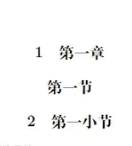
\includegraphics[width=8cm]{tu1.png}
    \caption{等比定律}
\end{figure}

第三段\par这说明\textbackslash par是可以强制分段的 %一般反斜杠需要引出其他指令,所以反斜杠是需要用\textbackslash输出的,单独的一个\加空格是空行

当然两个反斜杠\\也是可以强制分段的

\begin{figure}[htbp]
\centering
\subfigure[浮子的位移和速度随时间的关系图]{
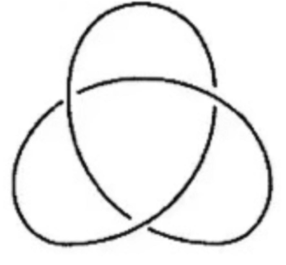
\includegraphics[width = .35\textwidth]{logo.png}
}
\quad
\subfigure[振子的位移和速度随时间的关系图]{
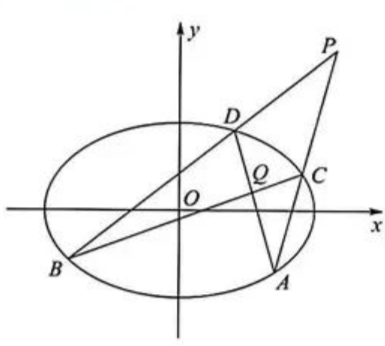
\includegraphics[width = .35\textwidth]{example.png}
}
\caption{情况2时的浮子与振子的垂荡位移和速度}
\end{figure}

\begin{description} %描述
\item[item 1] 描述1
\item[item 2] 描述2
\end{description}

\begin{table}[htbp]
\begin{center}

\setlength\tabcolsep{40pt}
表1\quad符号说明

\renewcommand{\arraystretch}{1.4}
\begin{tabular}{c c}
\hline
符号     & 含义                  \\ \hline
$E_i$ & 第$i$个企业     \\  
$r_i$      & 企业$E_i$的评价指标向量      \\  
$w$      & 层次分析法中的权重向量        \\  
$h_i$      & 企业$E_i$的信贷风险 \\ 
$\alpha_i$      &企业$E_i$的年利率         \\ 
$k$      & 不同类型的企业的受影响程度    \\ 
 \hline
\end{tabular}

\end{center}
\end{table}

根据问题一,可得:
\begin{equation}\label{阻尼}
F_\text{阻尼}=d_1\left(x^{'}(t)-X^{'}(t)\right).    
\end{equation}

则
\begin{equation}
P_\text{阻尼}=F_\text{阻尼}v_\text{相对}=d_1\left(x^{'}(t)-X^{'}(t)\right)^2.    
\end{equation}

问题四在问题二的基础上,增加了一个额外的做功装置——旋转阻尼器,
故而对于本问题的最大输出功率计算式,还需再考虑\eqref{阻尼},
此时也同样只需要考虑一个周期内整体系统的平均输出功率即可。

\end{document}